\documentclass[aspectratio=169,9pt,t]{beamer}

\usepackage[T1]{fontenc}
\usepackage{lmodern}
\usepackage{amsmath,amssymb,mathtools}
\usepackage{tikz}
\usetikzlibrary{arrows.meta,positioning,calc,fit,shapes.geometric}

% ---------- palette and Beamer setup ----------
\definecolor{Ink}{HTML}{172033}
\definecolor{Muted}{HTML}{5F6B7A}
\definecolor{Canvas}{HTML}{FAFAF7}
\definecolor{Graph}{HTML}{77736B}
\definecolor{BP}{HTML}{1769AA}
\definecolor{BPSoft}{HTML}{E8F2FA}
\definecolor{Gold}{HTML}{B85F00}
\definecolor{GoldSoft}{HTML}{FFF3D6}
\definecolor{Bad}{HTML}{B42318}

\usetheme{default}
\usefonttheme{professionalfonts}
\setbeamertemplate{navigation symbols}{}
\setbeamercolor{normal text}{fg=Ink,bg=Canvas}
\setbeamercolor{frametitle}{fg=Ink,bg=Canvas}
\setbeamercolor{statebar}{fg=Ink,bg=BPSoft}
\setbeamercolor{countbar}{fg=Ink,bg=white}
\setbeamercolor{explain}{fg=Ink,bg=white}
\setbeamercolor{takeaway}{fg=Ink,bg=GoldSoft}
\setbeamercolor{allocated}{fg=Ink,bg=BPSoft}
\setbeamercolor{temporary}{fg=Ink,bg=GoldSoft}
\setbeamersize{text margin left=6mm,text margin right=6mm}
\setbeamertemplate{frametitle}{%
  \vspace{.6mm}\insertframetitle\par
  \vspace{.2mm}{\color{Graph}\rule{\textwidth}{0.4pt}}\vspace{-2.2mm}}
\setbeamertemplate{footline}{%
  \leavevmode\hbox{%
    \begin{beamercolorbox}[wd=.84\paperwidth,ht=2.5ex,dp=1.1ex,leftskip=6mm]{normal text}%
      \fontsize{5.8}{6.6}\selectfont\color{Muted}%
      Memory: $L[3]$ + two arrays$[4+4]$ = 11 positions; slide 4 briefly uses one temporary variable (peak 12); graph/address data and hard decisions excluded
    \end{beamercolorbox}%
    \begin{beamercolorbox}[wd=.16\paperwidth,ht=2.5ex,dp=1.1ex,rightskip=6mm plus 1fil]{normal text}%
      \fontsize{6.2}{7.0}\selectfont\color{Muted}%
      Slide \insertframenumber\ of \inserttotalframenumber
    \end{beamercolorbox}}}

% ---------- fixed slide grammar ----------
\newcommand{\countstrip}[4]{%
  \begin{columns}[T,onlytextwidth]
    \column{.695\textwidth}
      \begin{beamercolorbox}[rounded=true,sep=.62ex]{statebar}
        \fontsize{6.4}{7.0}\selectfont\textcolor{Muted}{\bfseries STATE NOW}\par
        \vspace{.15ex}\scriptsize #1
      \end{beamercolorbox}
    \column{.285\textwidth}
      \begin{beamercolorbox}[rounded=true,sep=.52ex]{countbar}
        \fontsize{6.4}{7.0}\selectfont\textcolor{BP}{\bfseries MEMORY NOW}\par
        \fontsize{5.9}{6.6}\selectfont
        fixed $L$: 3 \quad current $U$: 4\par
        other array$[4]$: #2\par
        temporary variable: #3\par
        \textbf{values in use: #4}\quad arrays: 11 positions
      \end{beamercolorbox}
  \end{columns}\vspace{.6mm}}

\newcommand{\phase}[1]{%
  \centering\colorbox{GoldSoft}{\strut\scriptsize\bfseries\textcolor{Gold}{#1}}\par\vspace{1mm}}

\newcommand{\callout}[1]{%
  \begin{beamercolorbox}[rounded=true,sep=.65ex]{explain}
    \scriptsize #1
  \end{beamercolorbox}}

\newcommand{\takeaway}[1]{%
  \vspace{.6mm}\begin{beamercolorbox}[wd=\textwidth,rounded=true,sep=.6ex]{takeaway}
    \centering\scriptsize\bfseries #1
  \end{beamercolorbox}}

% ---------- diagram vocabulary ----------
\tikzset{
  bit/.style={circle,draw=BP,fill=white,line width=1.15pt,minimum size=8.5mm,inner sep=0pt,font=\scriptsize\bfseries},
  check/.style={rectangle,draw=BP,fill=BPSoft,line width=1.15pt,minimum width=8.5mm,minimum height=7.5mm,rounded corners=1.3pt,inner sep=0pt,font=\scriptsize\bfseries},
  edge/.style={draw=Graph!55,line width=1.1pt},
  activeedge/.style={draw=BP!35,line width=3.1pt},
  qmsg/.style={draw=BP,line width=2.05pt,dashed,-{Stealth[length=2.3mm]},shorten <=4mm,shorten >=3.7mm},
  umsg/.style={draw=BP,line width=2.05pt,dashed,-{Stealth[length=2.3mm]},shorten <=3.7mm,shorten >=4mm},
  msglabel/.style={fill=white,draw=BP,rounded corners=1.6pt,inner xsep=1.7pt,inner ysep=1pt,font=\fontsize{6.5}{7}\selectfont,text=Ink},
  uchip/.style={fill=white,draw=BP,rounded corners=1.6pt,inner xsep=1.8pt,inner ysep=1pt,font=\fontsize{6.5}{7}\selectfont,text=Ink},
  qchip/.style={fill=BPSoft,draw=BP,dashed,rounded corners=1.6pt,inner xsep=1.8pt,inner ysep=1pt,font=\fontsize{6.5}{7}\selectfont,text=Ink},
  localchip/.style={fill=GoldSoft,draw=Gold,rounded corners=1.6pt,inner xsep=1.8pt,inner ysep=1pt,font=\fontsize{6.5}{7}\selectfont,text=Gold},
  badchip/.style={fill=white,draw=Bad,dashed,rounded corners=1.6pt,inner xsep=1.8pt,inner ysep=1pt,font=\fontsize{6.5}{7}\selectfont,text=Bad},
  flowretain/.style={draw=BP,fill=BPSoft,line width=1.1pt,rounded corners=2.5pt,minimum height=12mm,text width=31mm,align=center,font=\scriptsize},
  flowtemp/.style={draw=Gold,fill=GoldSoft,dashed,line width=1.1pt,rounded corners=2.5pt,minimum height=12mm,text width=31mm,align=center,font=\scriptsize},
  flowarrow/.style={draw=BP,line width=1.35pt,-{Stealth[length=2.5mm]}},
  looparrow/.style={draw=Gold,line width=1.25pt,-{Stealth[length=2.5mm]}}
}

\newcommand{\bpgraphbase}{%
  \node[check] (A) at (-1.7,1.65) {$A$};
  \node[check] (B) at ( 1.7,1.65) {$B$};
  \node[bit] (b1) at (-3.0,0) {bit 1};
  \node[bit] (b2) at ( 0.0,0) {bit 2};
  \node[bit] (b3) at ( 3.0,0) {bit 3};
  \draw[edge] (A)--(b1);
  \draw[edge] (A)--(b2);
  \draw[edge] (B)--(b2);
  \draw[edge] (B)--(b3);
  \node[below=3.5mm of b1,font=\tiny] {$L_1=-2.197$};
  \node[below=3.5mm of b2,font=\tiny] {$L_2=+0.405$};
  \node[below=3.5mm of b3,font=\tiny] {$L_3=+0.693$};
}

\newcommand{\uedges}[4]{%
  \node[uchip] at ($(A)!.55!(b1)$) {#1};
  \node[uchip] at ($(A)!.55!(b2)$) {#2};
  \node[uchip] at ($(B)!.55!(b2)$) {#3};
  \node[uchip] at ($(B)!.55!(b3)$) {#4};
}

\newcommand{\graphstart}{\begin{tikzpicture}[x=.92cm,y=.92cm]}
\newcommand{\graphend}{\end{tikzpicture}}

\begin{document}

% Slide 1
\begin{frame}{BP in one loop: \texorpdfstring{$Q$}{Q} goes up and \texorpdfstring{$U$}{U} comes down}
  \countstrip{\textbf{BETWEEN ITERATIONS: }the three channel LLRs stay fixed; four current edge-addressed $U$ values are carried into the next message-passing iteration.}{available}{none}{7}

  \phase{VARIABLE PHASE FORMS $Q^{(t)}$ \quad $\longrightarrow$ \quad CHECK PHASE FORMS $U^{(t)}$ \quad $\longrightarrow$ \quad REPEAT}

  \begin{columns}[T,onlytextwidth]
    \column{.41\textwidth}
      \centering
      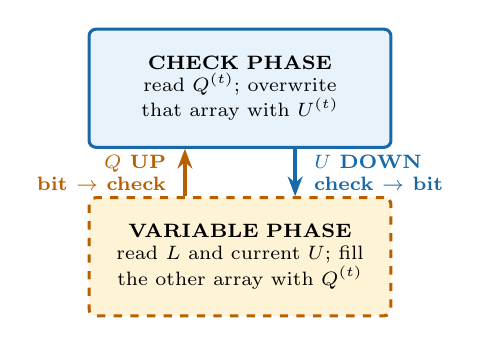
\begin{tikzpicture}[x=1cm,y=1cm]
        \node[flowretain,text width=36mm,minimum height=15mm] (check) at (0,1.12)
          {\textbf{CHECK PHASE}\\read $Q^{(t)}$; overwrite that array with $U^{(t)}$};
        \node[flowtemp,text width=36mm,minimum height=15mm] (variable) at (0,-1.02)
          {\textbf{VARIABLE PHASE}\\read $L$ and current $U$; fill the other array with $Q^{(t)}$};
        \draw[looparrow]
          ([xshift=-7mm]variable.north)--
          node[left=1mm,align=right,font=\scriptsize\bfseries,text=Gold]
            {$Q$ UP\\bit $\to$ check}
          ([xshift=-7mm]check.south);
        \draw[flowarrow]
          ([xshift=7mm]check.south)--
          node[right=1mm,align=left,font=\scriptsize\bfseries,text=BP]
            {$U$ DOWN\\check $\to$ bit}
          ([xshift=7mm]variable.north);
      \end{tikzpicture}
    \column{.57\textwidth}
      \callout{\centering\textbf{Variable-to-check rule}\par
        \[
          Q^{(t)}_{i\to c}
            =L_i+\sum_{d\in N(i)\setminus\{c\}}
                      U^{(t-1)}_{d\to i}
        \]
        Fixed $L_i$ plus information from checks other than the recipient.}
      \vspace{1mm}
      \callout{\centering\textbf{The two checks in this example have degree two}\par
        Each outgoing $U$ equals the other incoming $Q$.}
  \end{columns}

  \takeaway{Two four-position arrays exchange roles. One holds current $U$; the other holds $Q$ and is then overwritten by new $U$. A temporary variable performs each degree-two pair swap.}
\end{frame}

% Slide 2
\begin{frame}{Initialize once: channel LLRs and four edge addresses}
  \countstrip{\textbf{INITIAL VALUES: }fixed $\mathbf L=(-2.197,+0.405,+0.693)$ and current $\mathbf U^{(0)}=(0,0,0,0)$. No $Q$ value has been formed yet.}{available}{none}{7}

  \phase{PLACE THREE FIXED CHANNEL LLRS \quad + \quad INITIALIZE FOUR CURRENT $U$ VALUES}

  \begin{columns}[T,onlytextwidth]
    \column{.58\textwidth}
      \centering
      \graphstart
        \bpgraphbase
        \uedges{$U^{(0)}_{A\to1}=0$}{$U^{(0)}_{A\to2}=0$}{$U^{(0)}_{B\to2}=0$}{$U^{(0)}_{B\to3}=0$}
      \graphend
    \column{.40\textwidth}
      \callout{\centering
        \[
          L_i=\log\frac{p(y_i\mid b_i=1)}
                        {p(y_i\mid b_i=0)}
        \]
        Positive $L_i$ favours bit 1 under this deck's sign convention.}
      \vspace{1mm}
      \begin{beamercolorbox}[rounded=true,sep=.75ex]{allocated}
        \scriptsize\textcolor{BP}{\bfseries ELEVEN ARRAY POSITIONS; SEVEN VALUES IN USE NOW}\par\vspace{.4mm}
        \fontsize{7.0}{8.0}\selectfont
        $L[3]$ \hfill fixed throughout the decode\par
        current$[4]=U^{(0)}$ \hfill carried forward\par
        other$[4]$ \hfill available; next $Q^{(1)}$, then $U^{(1)}$\par
        temporary variable \hfill used only while converting $Q$ to $U$\par
        \textbf{array positions: 11} \hfill \textbf{check-phase peak: 12}
      \end{beamercolorbox}
  \end{columns}

\end{frame}

% Slide 3
\begin{frame}{Variable phase: all four \texorpdfstring{$Q^{(1)}$}{Q(1)} messages rise together}
  \countstrip{\textbf{FROZEN READ: }all four $Q^{(1)}$ values use the same current $\mathbf U^{(0)}$ and fill the other array. Checks A and B are shown together; neither consumes the other's new result.}{$Q^{(1)}[4]$}{none}{11}

  \phase{READ FIXED $L$ AND CURRENT $U^{(0)}$ \quad $\longrightarrow$ \quad FILL THE OTHER ARRAY$[4]$ WITH $Q^{(1)}$}

  \begin{columns}[T,onlytextwidth]
    \column{.56\textwidth}
      \centering
      \graphstart
        \bpgraphbase
        \draw[activeedge] (b1)--(A); \draw[activeedge] (b2)--(A);
        \draw[activeedge] (b2)--(B); \draw[activeedge] (b3)--(B);
        \node[draw=Gold,circle,line width=1.4pt,minimum size=10.5mm,inner sep=0pt] at (b2.center) {};
        \draw[qmsg] (b1)--node[msglabel,pos=.48,left=.7mm] {$-2.197$}(A);
        \draw[qmsg] (b2)--node[msglabel,pos=.50,left=.7mm] {$+0.405$}(A);
        \draw[qmsg] (b2)--node[msglabel,pos=.50,right=.7mm] {$+0.405$}(B);
        \draw[qmsg] (b3)--node[msglabel,pos=.48,right=.7mm] {$+0.693$}(B);
      \graphend
    \column{.42\textwidth}
      \[
        Q^{(1)}_{i\to c}
          =L_i+\sum_{d\in N(i)\setminus\{c\}}
                    U^{(0)}_{d\to i}
      \]
      \callout{\centering
        $\begin{aligned}
          Q^{(1)}_{1\to A}&=-2.197,&
          Q^{(1)}_{2\to A}&=+0.405,\\
          Q^{(1)}_{2\to B}&=+0.405,&
          Q^{(1)}_{3\to B}&=+0.693.
        \end{aligned}$}
      \vspace{1mm}
      \begin{beamercolorbox}[rounded=true,sep=.65ex]{takeaway}
        \centering\scriptsize\bfseries
        Degree-one bits have no other check:\par
        $Q^{(t)}_{1\to A}=L_1$ and $Q^{(t)}_{3\to B}=L_3$ for every $t$.
      \end{beamercolorbox}
  \end{columns}

  \takeaway{Every outgoing $Q$ begins with the fixed $L_i$ and adds only current $U$ values from checks other than its recipient.}
\end{frame}

% Slide 4
\begin{frame}{Check phase: both checks form all four \texorpdfstring{$U^{(1)}$}{U(1)} messages}
  \countstrip{\textbf{ONE CHECK-PHASE SNAPSHOT: }the other array changes from $Q^{(1)}[4]$ to $U^{(1)}[4]$. Each degree-two pair is read before those same two positions are overwritten.}{$Q^{(1)}\to U^{(1)}$}{1 during conversion}{12 peak}

  \phase{READ ONE $Q$ PAIR \quad $\longrightarrow$ \quad USE ONE TEMPORARY VARIABLE \quad $\longrightarrow$ \quad OVERWRITE THE SAME TWO POSITIONS WITH $U$}

  \begin{columns}[T,onlytextwidth]
    \column{.56\textwidth}
      \centering
      \graphstart
        \node[check] (A) at (-1.7,1.65) {$A$};
        \node[check] (B) at ( 1.7,1.65) {$B$};
        \node[bit] (b1) at (-3.0,0) {bit 1};
        \node[bit] (b2) at ( 0.0,0) {bit 2};
        \node[bit] (b3) at ( 3.0,0) {bit 3};
        \draw[edge] (A)--(b1); \draw[edge] (A)--(b2);
        \draw[edge] (B)--(b2); \draw[edge] (B)--(b3);
        \node[qchip] (q1a) at (-1.7,2.72) {$Q^{(1)}_{1\to A}=-2.197$};
        \node[qchip] (q2a) at (-1.7,2.25) {$Q^{(1)}_{2\to A}=+0.405$};
        \node[qchip] (q2b) at ( 1.7,2.72) {$Q^{(1)}_{2\to B}=+0.405$};
        \node[qchip] (q3b) at ( 1.7,2.25) {$Q^{(1)}_{3\to B}=+0.693$};
        \draw[activeedge] (A)--(b1); \draw[activeedge] (A)--(b2);
        \draw[activeedge] (B)--(b2); \draw[activeedge] (B)--(b3);
        \draw[umsg] (A)--node[msglabel,pos=.52,left=.7mm] {$+0.405$}(b1);
        \draw[umsg] (A)--node[msglabel,pos=.52,left=.7mm] {$-2.197$}(b2);
        \draw[umsg] (B)--node[msglabel,pos=.52,right=.7mm] {$+0.693$}(b2);
        \draw[umsg] (B)--node[msglabel,pos=.52,right=.7mm] {$+0.405$}(b3);
      \graphend
    \column{.42\textwidth}
      \begin{beamercolorbox}[rounded=true,sep=.65ex]{takeaway}
        \centering\scriptsize\bfseries
        DEGREE TWO: EACH OUTGOING $U$ IS THE OTHER INCOMING $Q$
      \end{beamercolorbox}
      \vspace{1mm}
      \begin{columns}[T,onlytextwidth]
        \column{.49\textwidth}
          \callout{\centering\textbf{check A}\par
            $\begin{aligned}
              U^{(1)}_{A\to1}&=+0.405,\\
              U^{(1)}_{A\to2}&=-2.197
            \end{aligned}$}
        \column{.49\textwidth}
          \callout{\centering\textbf{check B}\par
            $\begin{aligned}
              U^{(1)}_{B\to2}&=+0.693,\\
              U^{(1)}_{B\to3}&=+0.405
            \end{aligned}$}
      \end{columns}
      \vspace{.3mm}
      \callout{\centering
        \textbf{Same four positions; new quantities}\par\vspace{.4mm}
        $[-2.197,+0.405\mid+0.405,+0.693]_{Q}$\par
        $\Downarrow$ swap each degree-two pair using one temporary variable\par
        $[+0.405,-2.197\mid+0.693,+0.405]_{U}$\par
        $Q$ and $U$ are different messages; only the positions are reused. After both checks, exchange the two array roles.}
  \end{columns}

\end{frame}

% Slide 5
\begin{frame}{\texorpdfstring{$\Lambda$}{Lambda} includes every neighboring check; outgoing \texorpdfstring{$Q$}{Q} excludes its recipient}
  \countstrip{\textbf{AFTER EXCHANGING ARRAY ROLES: }$\mathbf U^{(1)}$ is current. The other array temporarily holds the three $\Lambda^{(1)}$ values; one position remains available. The $L_i$ values stay fixed.}{$\Lambda^{(1)}[3]$ + 1 free}{none}{10}

  \phase{DECISION VALUE: INCLUDE EVERY NEIGHBOR \quad $\longrightarrow$ \quad OUTGOING $Q$: EXCLUDE THE RECIPIENT CHECK}

  \begin{columns}[T,onlytextwidth]
    \column{.46\textwidth}
      \begin{beamercolorbox}[rounded=true,sep=.9ex]{allocated}
        \centering\scriptsize\textcolor{BP}{\bfseries DECISION VALUE: ALL NEIGHBORS}\par\vspace{.6mm}
        $\displaystyle
          \Lambda_i^{(1)}
            =L_i+\sum_{c\in N(i)}U^{(1)}_{c\to i}$\par\vspace{.6mm}
        Includes every check joined to bit $i$. It is used for the current decision; the fixed $L_i$ remains unchanged.
      \end{beamercolorbox}
      \vspace{1mm}
      \begin{beamercolorbox}[rounded=true,sep=.9ex]{temporary}
        \centering\scriptsize\textcolor{Gold}{\bfseries OUTGOING TO $c$: OTHER CHECKS ONLY}\par\vspace{.6mm}
        $\displaystyle
          Q^{(2)}_{i\to c}
            =L_i+\sum_{d\in N(i)\setminus\{c\}}U^{(1)}_{d\to i}$\par\vspace{.6mm}
        $\displaystyle Q^{(2)}_{i\to c}=\Lambda_i^{(1)}-U^{(1)}_{c\to i}$
      \end{beamercolorbox}
    \column{.52\textwidth}
      \callout{\textbf{NO OTHER CHECK REMAINS --- bit 1 sends to A}\par\vspace{.4mm}
        $N(1)=\{A\}$, so $N(1)\setminus\{A\}=\varnothing$.\par
        \centering$\displaystyle Q^{(2)}_{1\to A}=L_1+0=L_1=-2.197$}
      \vspace{1mm}
      \callout{\textbf{CHECK B REMAINS --- bit 2 sends to A}\par\vspace{.4mm}
        $N(2)=\{A,B\}$, so $N(2)\setminus\{A\}=\{B\}$.\par
        \centering$\displaystyle
          Q^{(2)}_{2\to A}=L_2+U^{(1)}_{B\to2}=+1.099$}
      \vspace{1mm}
      \begin{beamercolorbox}[rounded=true,sep=.8ex]{takeaway}
        \centering\scriptsize\bfseries
        If no other check remains, the index set is empty and the summation contributes zero. If another check remains, its $U$ value is included.
      \end{beamercolorbox}
  \end{columns}

\end{frame}

% Slide 6
\begin{frame}{Second variable phase: one bit sends two recipient-specific values}
  \countstrip{\textbf{FROZEN READ: }fixed $\mathbf L$ and current $\mathbf U^{(1)}$ fill the other array with all four $Q^{(2)}$ values.}{$Q^{(2)}[4]$}{none}{11}

  \phase{SAME BIT AND SAME $L_2$ \quad + \quad DIFFERENT RECIPIENT EXCLUSION \quad = \quad DIFFERENT $Q$}

  \begin{columns}[T,onlytextwidth]
    \column{.57\textwidth}
      \centering
      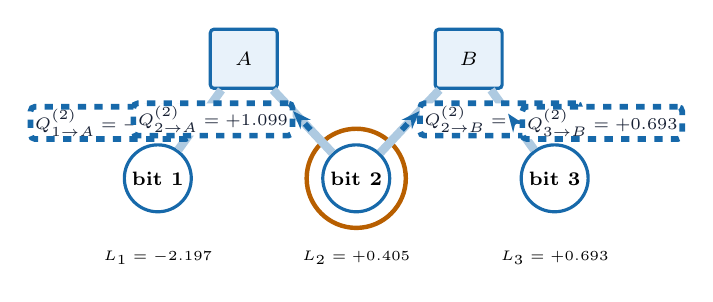
\begin{tikzpicture}[x=.84cm,y=.92cm]
        \bpgraphbase
        \node[draw=Gold,circle,line width=1.6pt,minimum size=11mm,fit=(b2),inner sep=0pt] {};
        \draw[activeedge] (b1)--(A); \draw[activeedge] (b2)--(A);
        \draw[activeedge] (b2)--(B); \draw[activeedge] (b3)--(B);
        \draw[qmsg] (b1)--node[msglabel,pos=.45,left=.6mm] {$Q^{(2)}_{1\to A}=-2.197$}(A);
        \draw[qmsg] (b2)--node[msglabel,pos=.53,left=.7mm] {$Q^{(2)}_{2\to A}=+1.099$}(A);
        \draw[qmsg] (b2)--node[msglabel,pos=.53,right=.7mm] {$Q^{(2)}_{2\to B}=-1.792$}(B);
        \draw[qmsg] (b3)--node[msglabel,pos=.45,right=.6mm] {$Q^{(2)}_{3\to B}=+0.693$}(B);
      \end{tikzpicture}
    \column{.41\textwidth}
      \callout{\centering\textbf{to check A: remove A's preceding contribution}\par
        \(
          Q^{(2)}_{2\to A}
            =\Lambda^{(1)}_2-U^{(1)}_{A\to2}
            =+1.099
        \)}
      \vspace{.4mm}
      \callout{\centering\textbf{to check B: remove B's preceding contribution}\par
        \(
          Q^{(2)}_{2\to B}
            =\Lambda^{(1)}_2-U^{(1)}_{B\to2}
            =-1.792
        \)}
      \vspace{.4mm}
      \begin{beamercolorbox}[rounded=true,sep=.65ex]{takeaway}
        \centering\scriptsize\bfseries
        $Q^{(2)}_{2\to A}\ne Q^{(2)}_{2\to B}$ even though both originate at bit 2.
      \end{beamercolorbox}
  \end{columns}

  \takeaway{The edge address determines which preceding check-to-variable value is excluded.}
\end{frame}

% Slide 7
\begin{frame}{What remains between iterations, and how the two arrays exchange roles}
  \countstrip{\textbf{BETWEEN ITERATIONS: }the three $L$ values remain fixed and four current $U^{(t)}$ values are carried forward. $Q$ and $\Lambda$ do not need to remain.}{available}{none}{7}

  \phase{FILL THE OTHER ARRAY WITH $Q$ \quad $\longrightarrow$ \quad OVERWRITE IT WITH NEW $U$ \quad $\longrightarrow$ \quad EXCHANGE ARRAY ROLES}

  \begin{columns}[T,onlytextwidth]
    \column{.43\textwidth}
      \centering
      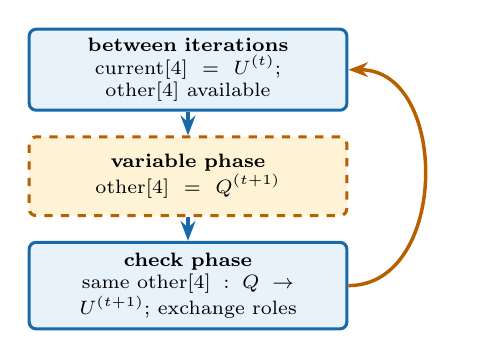
\begin{tikzpicture}[node distance=3mm]
        \node[flowretain,text width=38mm,minimum height=10mm] (old)
          {\textbf{between iterations}\\current$[4]=U^{(t)}$; other$[4]$ available};
        \node[flowtemp,text width=38mm,minimum height=10mm,below=of old] (q)
          {\textbf{variable phase}\\other$[4]=Q^{(t+1)}$};
        \node[flowretain,text width=38mm,minimum height=11mm,below=of q] (new)
          {\textbf{check phase}\\same other$[4]:Q\to U^{(t+1)}$; exchange roles};
        \draw[flowarrow] (old)--(q);
        \draw[flowarrow] (q)--(new);
        \draw[looparrow] (new.east) to[out=0,in=0,looseness=1.20] (old.east);
      \end{tikzpicture}
      \vspace{1mm}
      \begin{beamercolorbox}[rounded=true,sep=.8ex]{takeaway}
        \centering\scriptsize
        Between phases, the other array may hold the three $\Lambda$ values used for the current decision; it is then reused for the next $Q[4]$.
      \end{beamercolorbox}
    \column{.55\textwidth}
      \begin{beamercolorbox}[rounded=true,sep=.8ex]{allocated}
        \scriptsize\textcolor{BP}{\bfseries ARRAY POSITIONS KEPT THROUGHOUT THE DECODE}\par\vspace{.5mm}
        \fontsize{7.2}{8.3}\selectfont
        $L[3]$ \hfill 3 fixed number positions\par
        array A$[4]$ \hfill 4 positions\par
        array B$[4]$ \hfill 4 positions\par
        A and B exchange current/other roles\par
        \textbf{total array positions} \hfill \textbf{11}
      \end{beamercolorbox}
      \vspace{1mm}
      \begin{beamercolorbox}[rounded=true,sep=.8ex]{temporary}
        \scriptsize\textcolor{Gold}{\bfseries VALUES IN USE AT EACH STAGE}\par\vspace{.5mm}
        \fontsize{7.2}{8.3}\selectfont
        between iterations: $3L+4U=7$\par
        while the other array holds $Q$: $3+4+4=11$\par
        one temporary variable during a degree-two pair conversion\par
        \textbf{maximum in use: $3+4+4+1=12$}\par
        optional hard-decision estimate: 3 bits, counted separately\par
        this degree-two reuse schedule is not a universal BP memory bound
      \end{beamercolorbox}
  \end{columns}
\end{frame}

\end{document}
